\documentclass[main.tex]{subfiles}
\begin{document}
\subsection{Day 40: 11/30/22}
\subsubsection{Inverse Function Theorem}

To provide some motivation, we first consider the single-variable case. Suppose $f:\parens{a - r, a + r}\to \RR$ is $C^1$ and $f'(a) \neq 0$ (WLOG $> 0$).

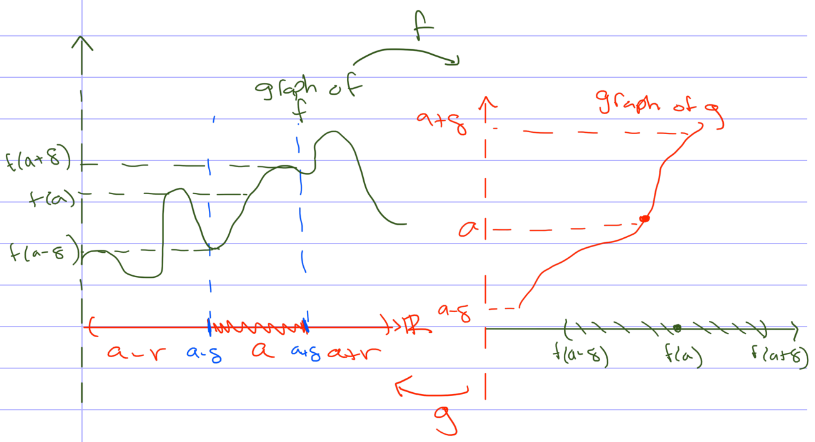
\includegraphics[width = 0.9\textwidth]{inverse_function_theorem.PNG}

Since $f'(a) > 0$ and $f'$ is continuous ($C^1$) there exists $\delta \in (0, r)$ such that $f'(x) > 0$ for all $x\in (a - \delta, a + \delta)$. By MVT, this implies that $f$ is strictly increasing on this interval, so $f$ must be bijective from $(a - \delta, a + \delta)$ to $(f(a - \delta), f(a + \delta))$. Thus, we can define the function $g = \parens{f |_{(a - \delta, a + \delta)}}^{-1} : (f(a - \delta), f(a + \delta)) \to (a - \delta, a + \delta)$ as the inverse of $f$ (on $(a - \delta, a + \delta)$), which is also differentiable.

Then for all $y\in (f(a - \delta), f(a + \delta)$, we have
\begin{align*}
    &f(g(y)) = y \\
    &\implies f'(g(y))g'(y) = 1 \\
    &\implies g'(y) = \frac{1}{f'(g(y))};
\end{align*}
since $g'$ is the composition of $t\to \frac{1}{t}$, $f'$, and $g$ which are all continuous, it follows that $g'$ is continuous too so $g$ is $C^1$. Now let's move onto the general case:

\begin{theorem}[Inverse Function Theorem]
    Suppose $U\subseteq \RR^n$ is open, $\vf : U \to \RR^n$ is $C^1$, and $\mathcal{D}\vf\parens{\va}$ is an invertible $n\times n$ matrix at some $\va\in U$. Then there exists open sets $V\subseteq U$ containing $\va$ and $W\subseteq \RR^n$ containing $\vf(a)$ such that $\vf$ is bijective on $V$, $\vf(V) = W$, and the inverse $\vg = \parens{\vf |_V}^{-1} : W \to V$ is $C^1$.
\end{theorem}

\begin{remark}
    Observe that since $\vf$ and $\vg$ are both differentiable, it follows that for all $\vy\in W$, we have
    \[\vf\parens{\vg\parens{\vy}} = \vy \implies \mathcal{D}\vf\parens{\vg\parens{\vy}}\mathcal{D}\vg\parens{\vy} = I\]
    by Chain Rule and Problem Set 8 Problem 9. By Problem Set 13 Problem 1, this implies that $\mathcal{D}\vf\parens{\vg\parens{\vy}}$ is invertible with $\parens{\mathcal{D}\vf\parens{\vg\parens{\vy}}}^{-1} = \mathcal{D}\vg\parens{\vy}$ for all $\vy\in W$.
\end{remark}

\begin{proof}
    Since $\va\in U$ and $U$ is open, there exists a $\sigma > 0$ such that $B_\sigma\parens{\va}\subseteq U$. Since $f$ is $C^1$, each of the $\mathcal{D}_if_j$ are continuous, so taking $\varepsilon_0 = \boxed{\frac{1}{2n\norm{\mathcal{D}\vf\parens{\va}^{-1}}}}$, we have a $\delta_{ij} > 0$ for each $i,j \in \braces{1, \ldots , n}$ such that $\abs{\mathcal{D}_if_j\parens{\vx} - \mathcal{D}_if_j\parens{\va}} < \varepsilon_0$ for all $x\in U \cap B_{\delta_{ij}}\parens{\va}$. Define $\rho > 0$ as the minimum of $\sigma$ and all the $\delta_{ij}$. Then for all $\vx\in B_\rho\parens{\va}$ we have
    \[\norm{\mathcal{D}\vf\parens{\vx} - \mathcal{D}\vf\parens{\va}}^2 = \sum_{i, j = 1}^n \abs{\mathcal{D}_if_j\parens{\vx} - \mathcal{D}_if_j\parens{\va}} < n^2\varepsilon_0^2.\]
    Define the error function $\mathrm{E} : B_\rho\parens{\va}\to \RR^n$ by $\mathrm{E}\parens{\vx} = \vf\parens{\vx} - \vf\parens{\va} - \mathcal{D}\vf\parens{\va}\parens{\vx - \va} = \vf\parens{\vx} - \mathcal{D}\vf\parens{\va}\vx - \vf\parens{\va} + \mathcal{D}\vf\parens{\va}\va$; the first term is differentiable by definition, the second is differentiable by Midterm 2, and the last two are both constants; thus, applying our knowledge of derivatives, we have $\mathcal{D}\mathrm{E}\parens{\vx} = \mathcal{D}\vf\parens{\vx} - \mathcal{D}\vf\parens{\va}$ for all $\vx\in B_\rho\parens{\va}$, and plugging this into our earlier equation, we arrive at $\norm{\mathcal{D}\mathrm{E}\parens{\vx}} < n\varepsilon_0$. By Problem Set 14 Problem 9, it then follows that for all $\vx, \vx'\in B_\rho\parens{\va}$, we have
    \begin{align*}
        &\norm{\mathrm{E}\parens{\vx} - \mathrm{E}\parens{\vx'}} \le n\varepsilon_0 \sqrt{n}\norm{\vx - \vx'} \\
        &\iff \norm{\parens{\vf\parens{\vx} - \mathcal{D}\vf\parens{\va}} - \parens{\vf\parens{\vx'} - \mathcal{D}\vf\parens{\va'}}} \le n\varepsilon_0 \sqrt{n}\norm{\vx - \vx'} \\
        &\iff \boxed{\norm{\vf\parens{\vx} - \vf\parens{\vx'} - \mathcal{D}\vf\parens{\va}\parens{\vx - \vx'}} \le n\varepsilon_0 \sqrt{n}\norm{\vx - \vx'}}.
    \end{align*}
    This implies that
    \begin{align*}
        &\norm{\mathcal{D}\vf\parens{\va}^{-1}\parens{\vf\parens{\vx} - \vf\parens{\vx'}} - \parens{\vx - \vx'}} \\
        &= \norm{\mathcal{D}\vf\parens{\va}^{-1}\parens{\vf\parens{\vx} - \vf\parens{\vx'} - \mathcal{D}\vf\parens{\va}\parens{\vx - \vx'}}} \\
        &\le \norm{\mathcal{D}\vf\parens{\va}^{-1}}\norm{\vf\parens{\vx} - \vf\parens{\vx'} - \mathcal{D}\vf\parens{\va}\parens{\vx - \vx'}} \\
        &\le \norm{\mathcal{D}\vf\parens{\va}^{-1}}n\varepsilon_0 \sqrt{n}\norm{\vx - \vx'} \\
        &= \norm{\mathcal{D}\vf\parens{\va}^{-1}}\cdot \frac{n\sqrt{n}}{2n^2\norm{\mathcal{D}\vf\parens{\va}^{-1}}}\norm{\vx - \vx'} \\
        &= \frac{1}{2\sqrt{n}}\norm{\vx - \vx'} \\
        &\le \frac{1}{2}\norm{\vx - \vx'}.
    \end{align*}
    Therefore, it follows that
    \begin{align*}
        \norm{\vx - \vx'} &= \norm{-\parens{\vx - \vx'}} \\
        &\le \norm{\mathcal{D}\vf\parens{\va}^{-1}\parens{\vf\parens{\vx} - \vf\parens{\vx'}} - \parens{\vx - \vx'}} + \norm{\mathcal{D}\vf\parens{\va}^{-1}\parens{\vf\parens{\vx} - \vf\parens{\vx'}}} \\
        &\le \frac{1}{2}\norm{\vx - \vx'} + \norm{\mathcal{D}\vf\parens{\va}^{-1}\parens{\vf\parens{\vx} - \vf\parens{\vx'}}},
    \end{align*}
    so $\frac{1}{2}\norm{\vx - \vx'} \le \norm{\mathcal{D}\vf\parens{\va}^{-1}\parens{\vf\parens{\vx} - \vf\parens{\vx'}}}$ for all $\vx, \vx'\in B_\rho\parens{\va}$. We continue this proof in the next lecture.
\end{proof}

\end{document}